\subsection{Introduction} 
%LET'S GO TEAM!!! ONE LESS SECTION
%We are unstoppppable --> DAB DAB DAB
In this chapter it is seen how the final constellation decision is made. To do that an analysis of weights will be performed.\\

The constellation candidates selected to their later evaluation are the following:

\subsection{Candidate 1: Polar - Global Coverage}

This polar constellation (Figure \ref{fig:Candidate1}) came from the street coverage method explained in \ref{PolarOrbit}. It is a network of polar orbits that provides global coverage. This constellation is generated as follows:

\begin{figure}%[H] %[b] % h / H / b / t
	\centering
	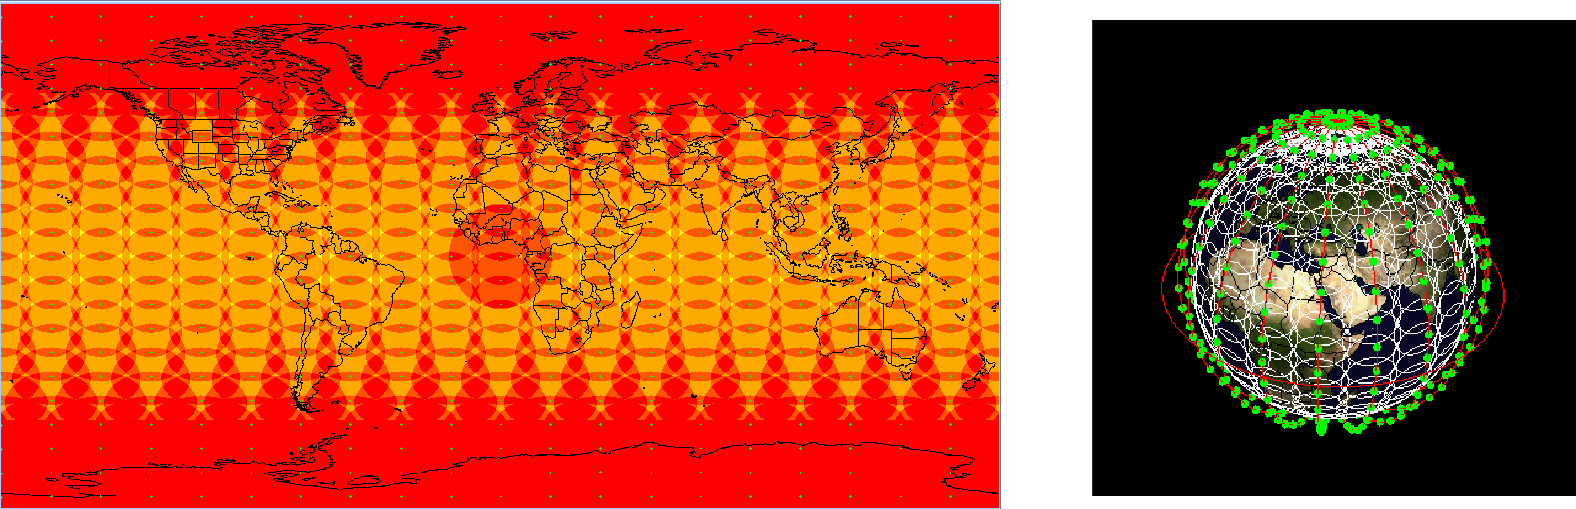
\includegraphics[width=1\textwidth]{Candidate1.png}\\
	\caption{Candidate 1. Full Polar constellation with global coverage.
			 h= 560km; Np=20; Npp=21; Tsat=420 }
	\label{fig:Candidate1}
\end{figure}


\subsection{Candidate 2: Polar - GS Coverage}
 
The second candidate that will be compared is a polar orbit extracted from the coverage method explained in \ref{PolarOrbit} (Figure \ref{fig:Candidate2}). This constellation provides total coverage to the Astrea's team ground stations. The constellation distribution is set as follows:

\begin{figure}%[H] %[b] % h / H / b / t
	\centering
	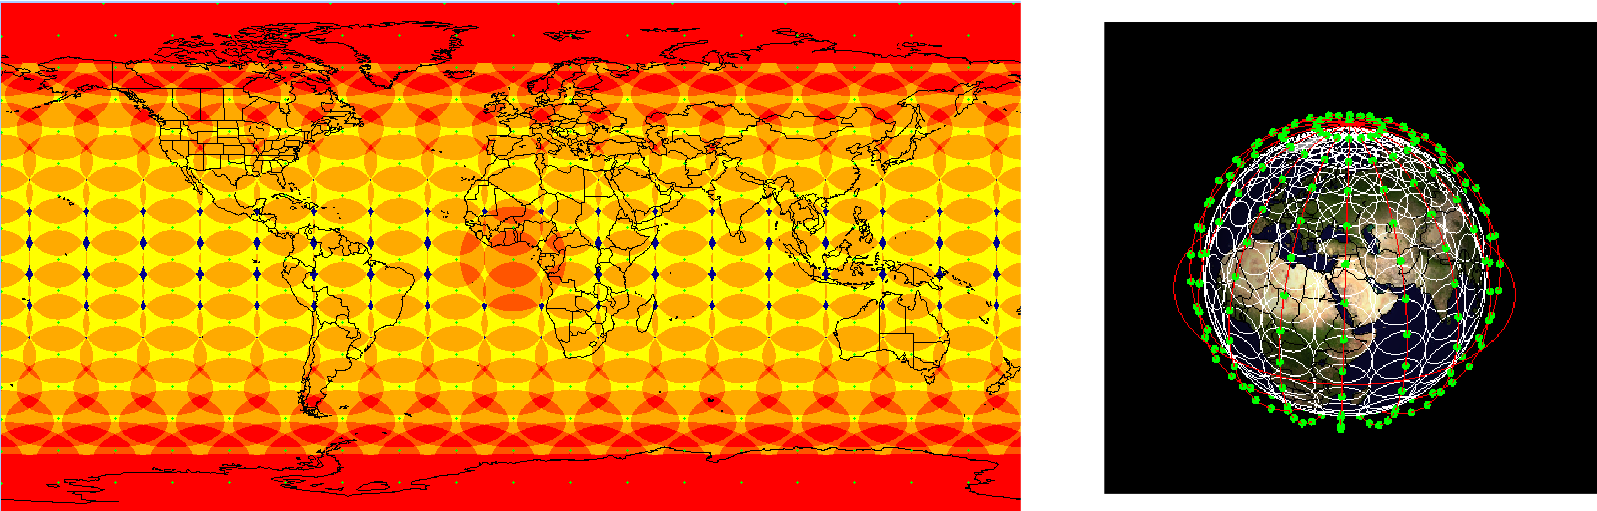
\includegraphics[width=1\textwidth]{Candidate2.png}\\
	\caption{Candidate 2. Full Polar constellation with total ground station coverage.
			 h= 550km; Np=18; Npp=20; Tsat=288 }
	\label{fig:Candidate2}
\end{figure}


\subsection{Candidate 3 and 4: Walker-Delta GS Coverage}

Two Walker-Delta constellation configurations have been also chosen due to their reduced number of planes and satellites while being able of providing total coverage on the lattitudes where the ground stations are located.(Figures \ref{fig:Candidate3} and \ref{fig:Candidate4}).
These constellations have been obtained with the algorithm explained in \ref{Testing}. The distribution of these constellations is described below:

\textbf{Candidate 3}\\

\begin{figure}%[H] %[b] % h / H / b / t
	\centering
	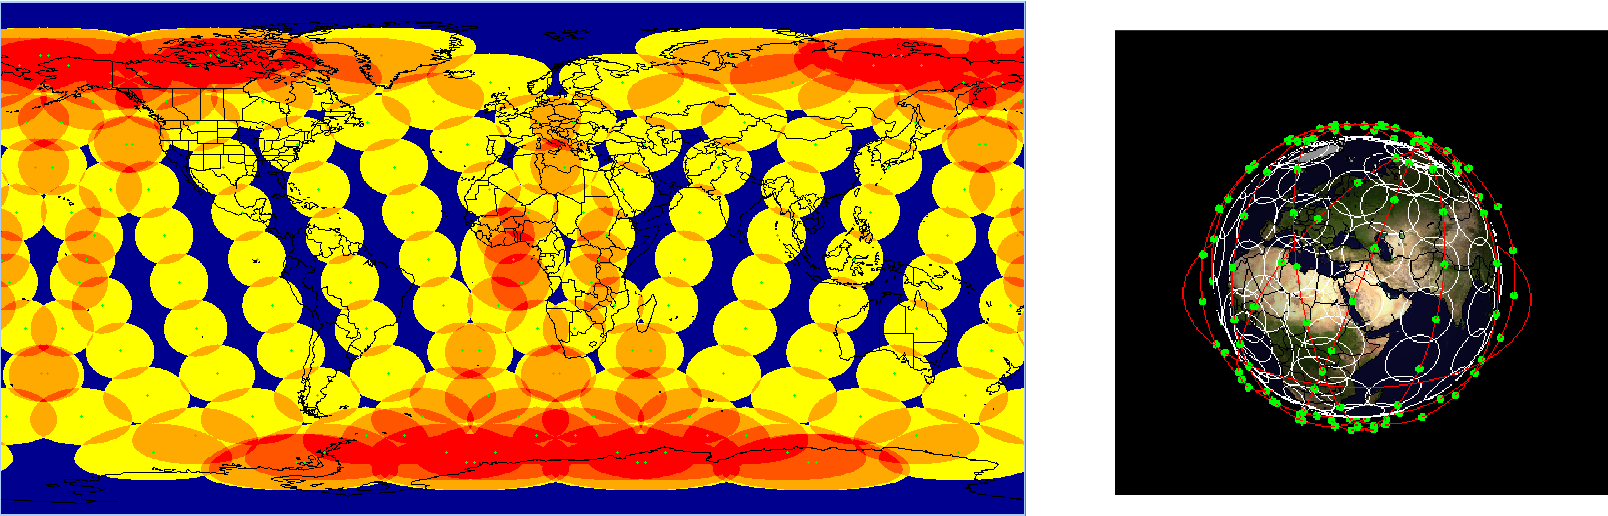
\includegraphics[width=1\textwidth]{Candidate3.png}\\
	\caption{Candidate 3. 210º Walker-Delta constellation configuration.
			 h= 542km; in=72; Np=8; Npp=21; Tsat=168 }
	\label{fig:Candidate3}
\end{figure}


\textbf{Candidate 4}\\  

\begin{figure}%[H] %[b] % h / H / b / t
	\centering
	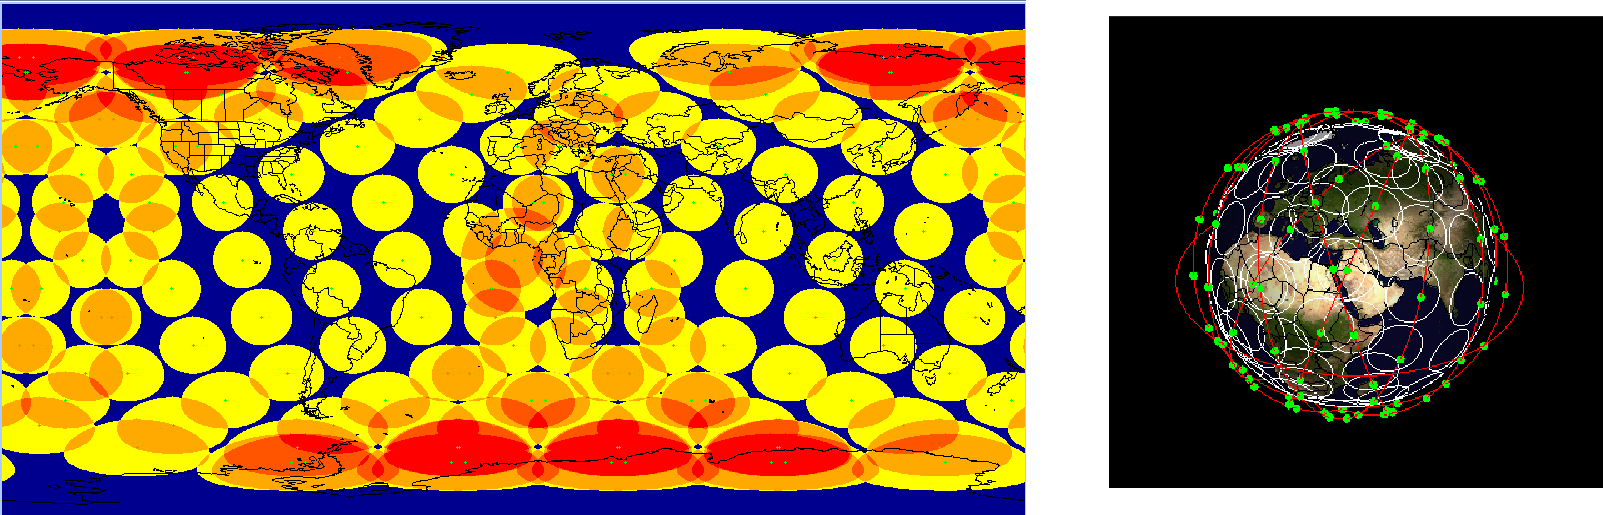
\includegraphics[width=1\textwidth]{Candidate4.png}\\
	\caption{Candidate 4. 225º Walker-Delta constellation configuration.
			 h= 542km; in=72; Np=9; Npp=17; Tsat= 153}
	\label{fig:Candidate4}
\end{figure}



\subsection{Candidate 5: Walker-Delta Lat: 0-58}

Another Walker-Delta constellation has been selected with the criteria of total coverage of a range of lattitudes going from 0 to 58 (Figure \ref{fig:Candidate5}). Therefore, the distribution needed to fulfill this particular condition of the constellation obtained from \ref{PerformanceAnal} is the following:

\begin{figure}%[H] %[b] % h / H / b / t
	\centering
	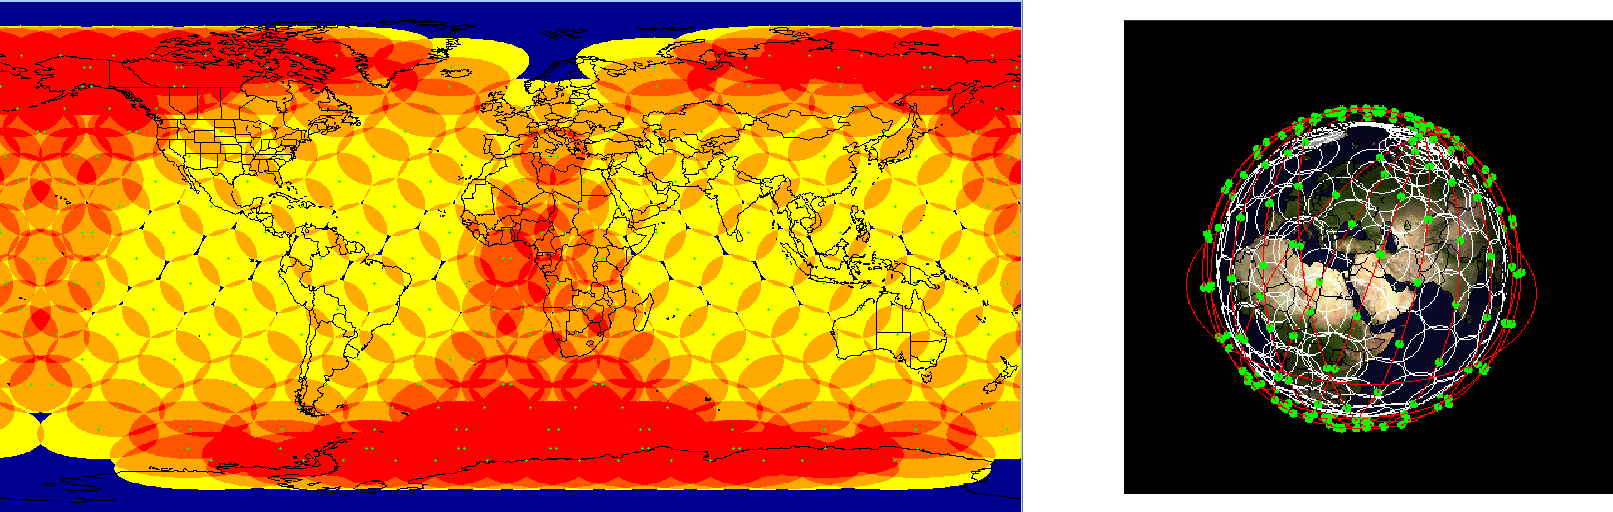
\includegraphics[width=1\textwidth]{Candidate5.png}\\
	\caption{Candidate 5. 210º Walker-Delta constellation configuration with total coverage of the latitudes from 0 to 52 degrees.
			 h= 560km; in=72; Np=14; Npp=19; Tsat= 226} 
	\label{fig:Candidate5}
\end{figure}


\subsection{Candidate 6: Polar - Walker-Delta J2 + Rotació}

With the goal of providing constant coverage at the Ground Stations we can design a constellation that takes profit of the rotation of the Earth. If we also consider Earth's oblateness that causes another $\Omega$ derivative with time, we can exacty compute the longitudinal position of a plane after an orbit has passed. Now, if we design the constellation in a way that this deviation after an orbit matches the separation between planes, a line of satellites will always be on the GS. (Figure \ref{fig:Candidate6})

\begin{figure}%[H] %[b] % h / H / b / t
	\centering
	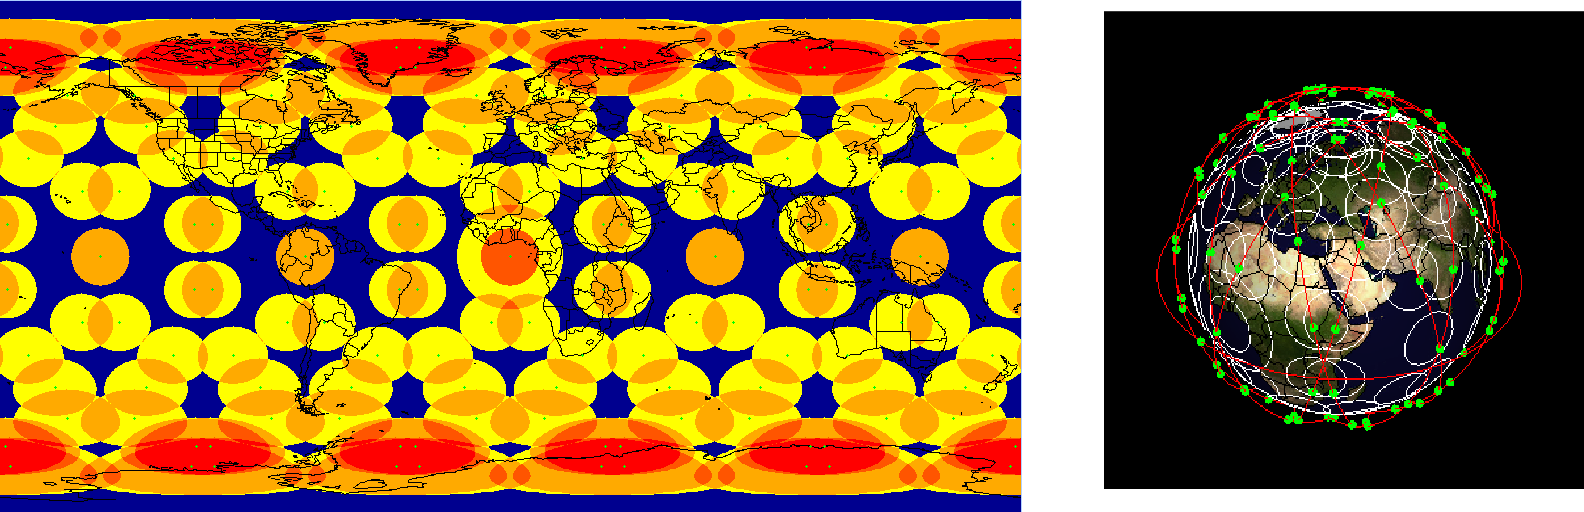
\includegraphics[width=1\textwidth]{Candidate6.png}\\
	\caption{Candidate 6. 225º Walker-Delta constellation configuration. h= 542km; in=72; Np=14; Npp=19; Tsat= 226}
	\label{fig:Candidate6}
\end{figure}

\subsection{Candidate 7: Walker-Delta GS Coverage 3}

The last configuration to be studied is a Walker-Delta constellation configuration designed to provide total coverage to the ground stations (Figure \ref{fig:Candidate7}). It came up from candidate 3 constellation adding one more plane in order to increase its global coverage and minimize the gaps. As can be seen below, its parameters are the same as candidate 3 adding an extra plane.

\begin{figure}%[H] %[b] % h / H / b / t
	\centering
	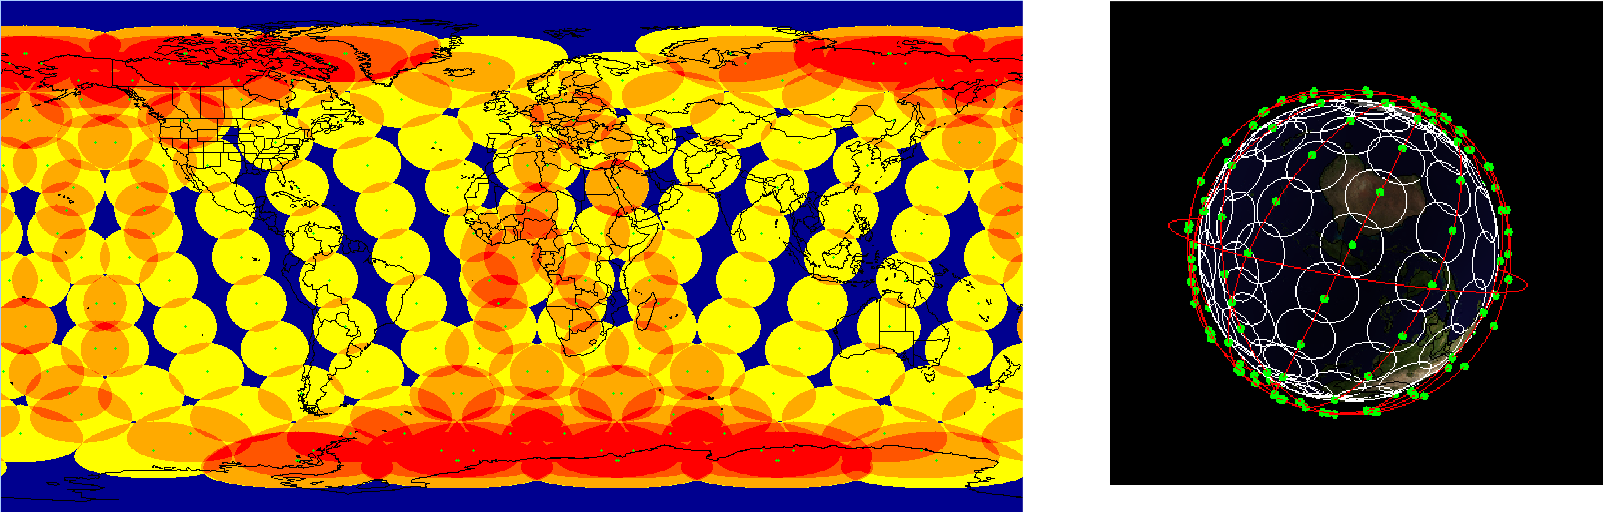
\includegraphics[width=1\textwidth]{Candidate7.png}\\
	\caption{Candidate 7. Full Walker-Delta constellation configuration.h= 542km; in=72; Np=9; Npp=21; Tsat= 189}
	\label{fig:Candidate7}
\end{figure}

\subsection{Final candidate constellation paramater comparison.}


The different parameters for the 7 candidate constellations are defined in table \ref{candidateparameters}. These are essential in order to compute further calculations regarding the final constellation design. 


\begin{table}[h]
\centering
\begin{tabular}{ | c | c | c | c | c | c | c | c | }
\hline
	
	\textbf{Candidates} & \textbf{1} & \textbf{2} & \textbf{3} & \textbf{4} & \textbf{5} & \textbf{6} & \textbf{7} \\ \hline
	Height of the satellites(km) & 560 & 550 & 542 & 542 & 560 & 542 & 542 \\ \hline
	Inclinations of the plane (deg) & 90 & 90 & 72 & 72 & 72 & 72 & 72 \\ \hline
	Number of planes & 20 & 18 & 8 & 9 & 14 & 14 & 9 \\ \hline
	Satellites per plane & 21 & 16 & 21 & 17 & 19 & 19 & 21 \\ \hline
	Total number of satellites & 420 & 288 & 168 & 153 & 226 & 226 & 189\\ \hline
	Range of argument of ascending node(deg)& 360 & 360 & 210 & 225 & 210 & 210 & 225 \\ \hline
	
\end{tabular}
\caption{Key parameters of the different candidate constellations}\label{candidateparameters}
\end{table}


